\subsubsection{Increasing destination size}

In this experiment, we also use a partition of 2014 nodes. In which, we keep the number of source nodes constant (64 nodes) and increase the number of destination nodes starting from 128 to 256, 512 and 1024 nodes. Each source node communicates with k destination nodes with k = 2, 4, 8 and 16 respectively. In detail, a node id x communicates with node ids (k*x, k*x+1, ..., k*x+k-1). There is 1 MPI/PAMI rank per node. Each pair of communication transfers 8 MB of data. We experimented with 3 approaches Optimization, Heuristics and MPI\_Alltoallv for 3 patterns Disjoint, Overlap and Subset. The performance is shown in Figure \ref{fig:incrsize}.

\begin{figure*}[!htbp]
        \centering
        \begin{subfigure}[b]{0.32\textwidth}
                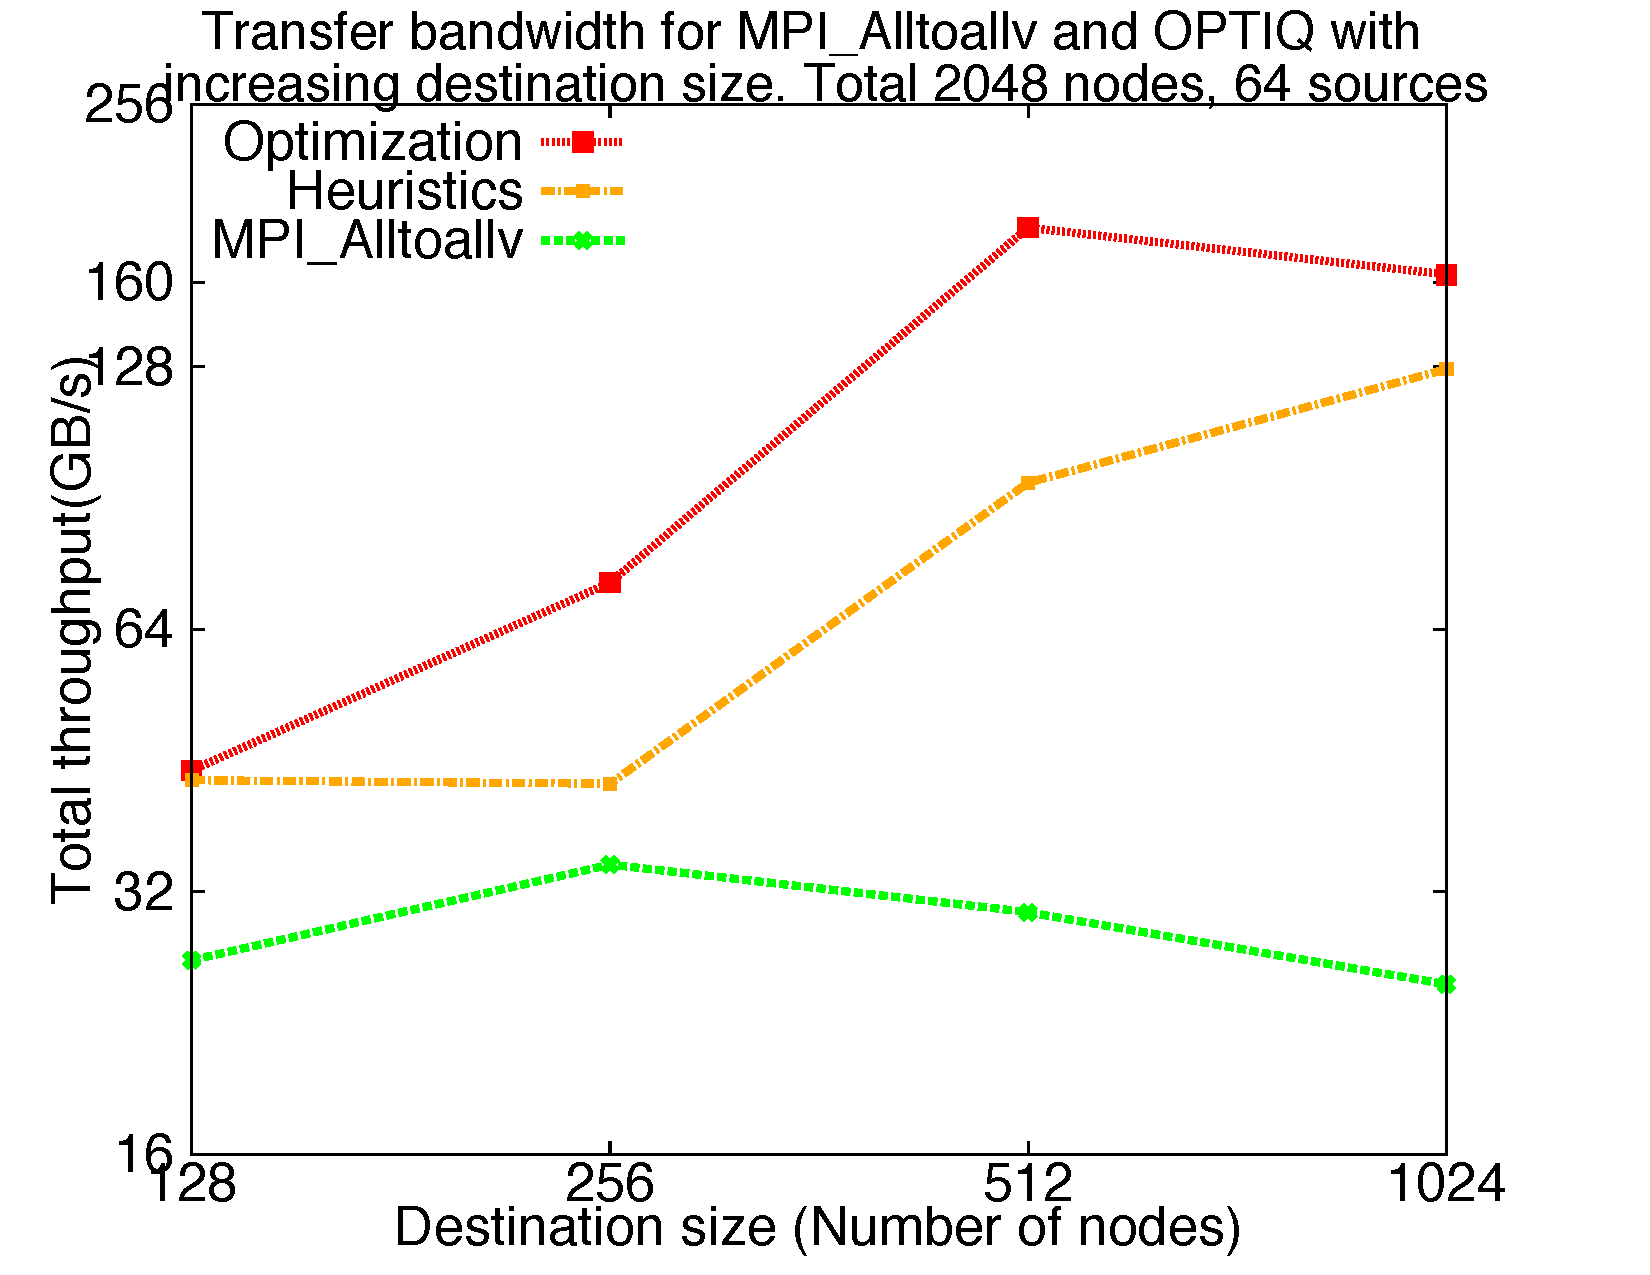
\includegraphics[width=\textwidth]{figures/incrsize_disjoint.pdf}
                \caption{Disjoint}
                \label{fig:incrsize_disjoint}
        \end{subfigure}%
        ~ %add desired spacing between images, e. g. ~, \quad, \qquad, \hfill etc.
          %(or a blank line to force the subfigure onto a new line)
        \begin{subfigure}[b]{0.32\textwidth}
                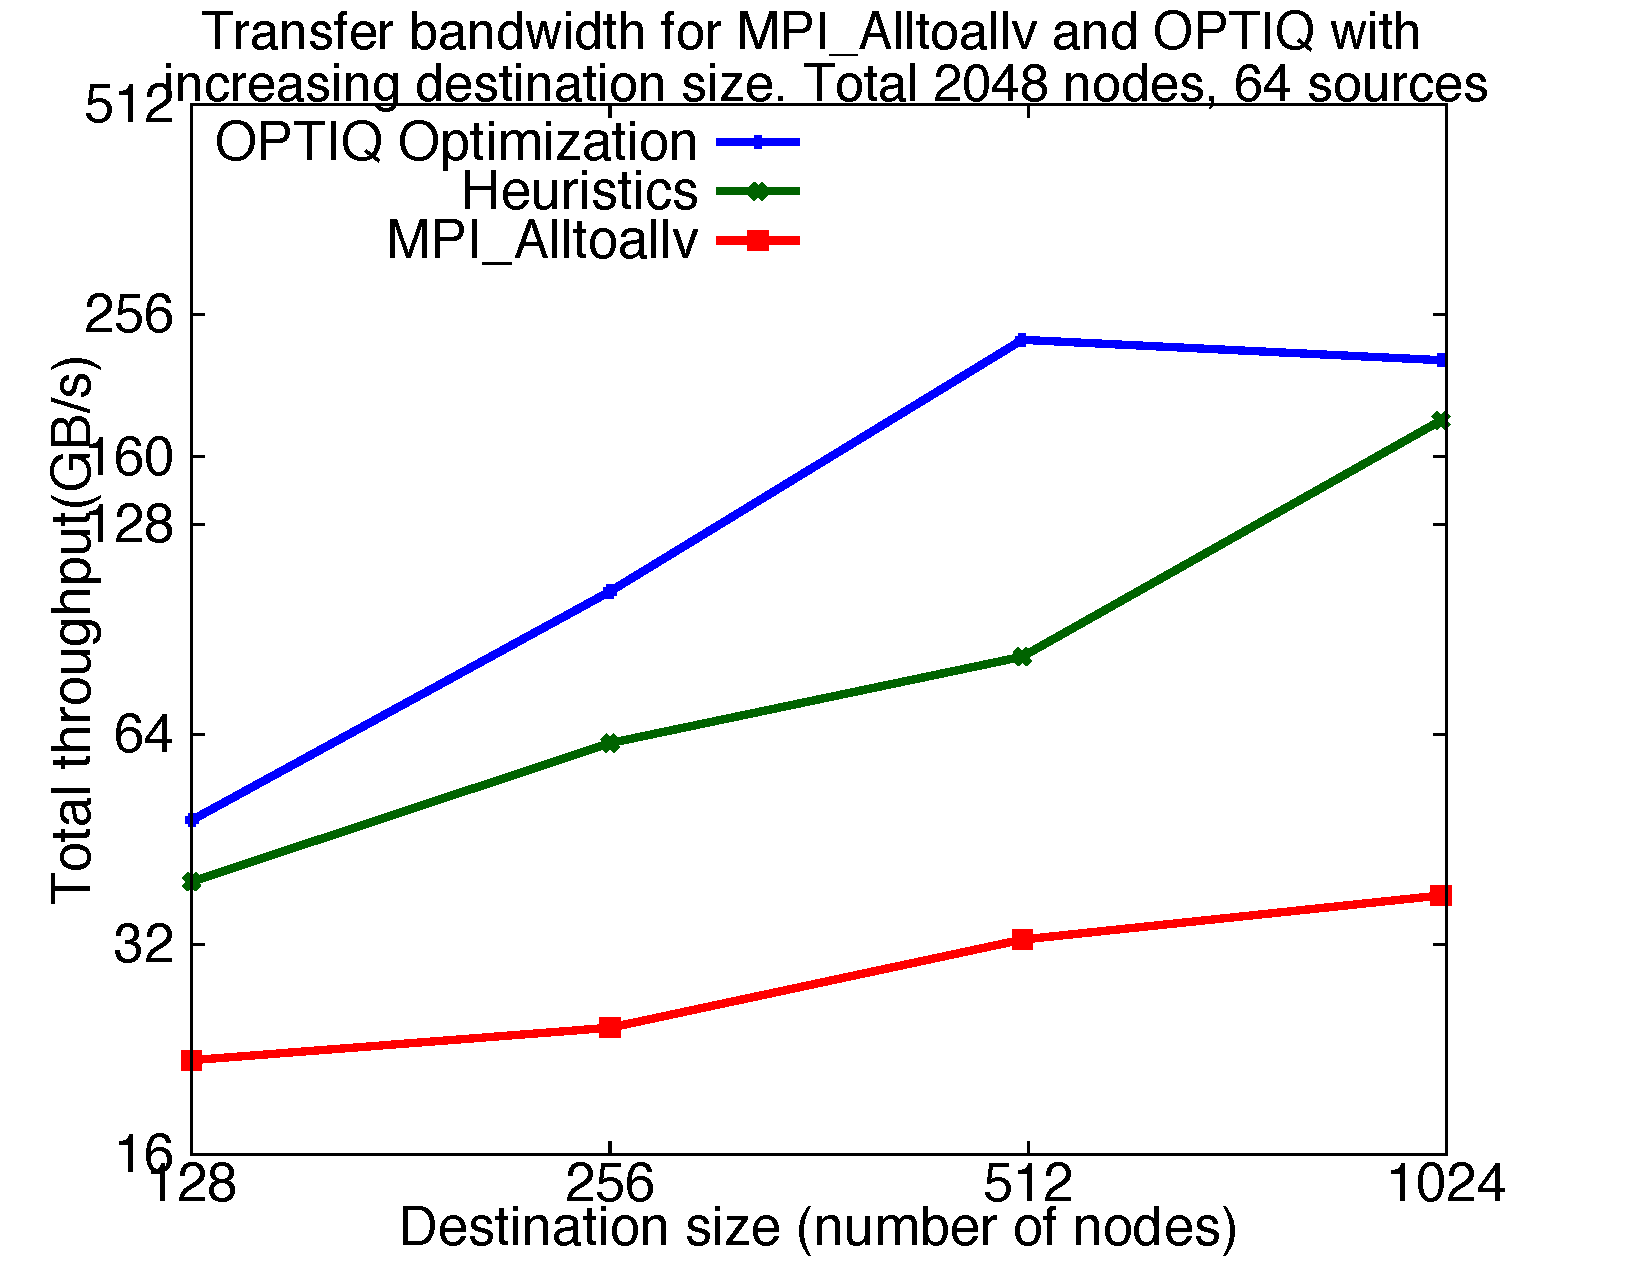
\includegraphics[width=\textwidth]{figures/incrsize_overlap}
                \caption{Overlap}
                \label{fig:incrsize_overlap}
        \end{subfigure}
        ~ %add desired spacing between images, e. g. ~, \quad, \qquad, \hfill etc.
          %(or a blank line to force the subfigure onto a new line)
        \begin{subfigure}[b]{0.32\textwidth}
                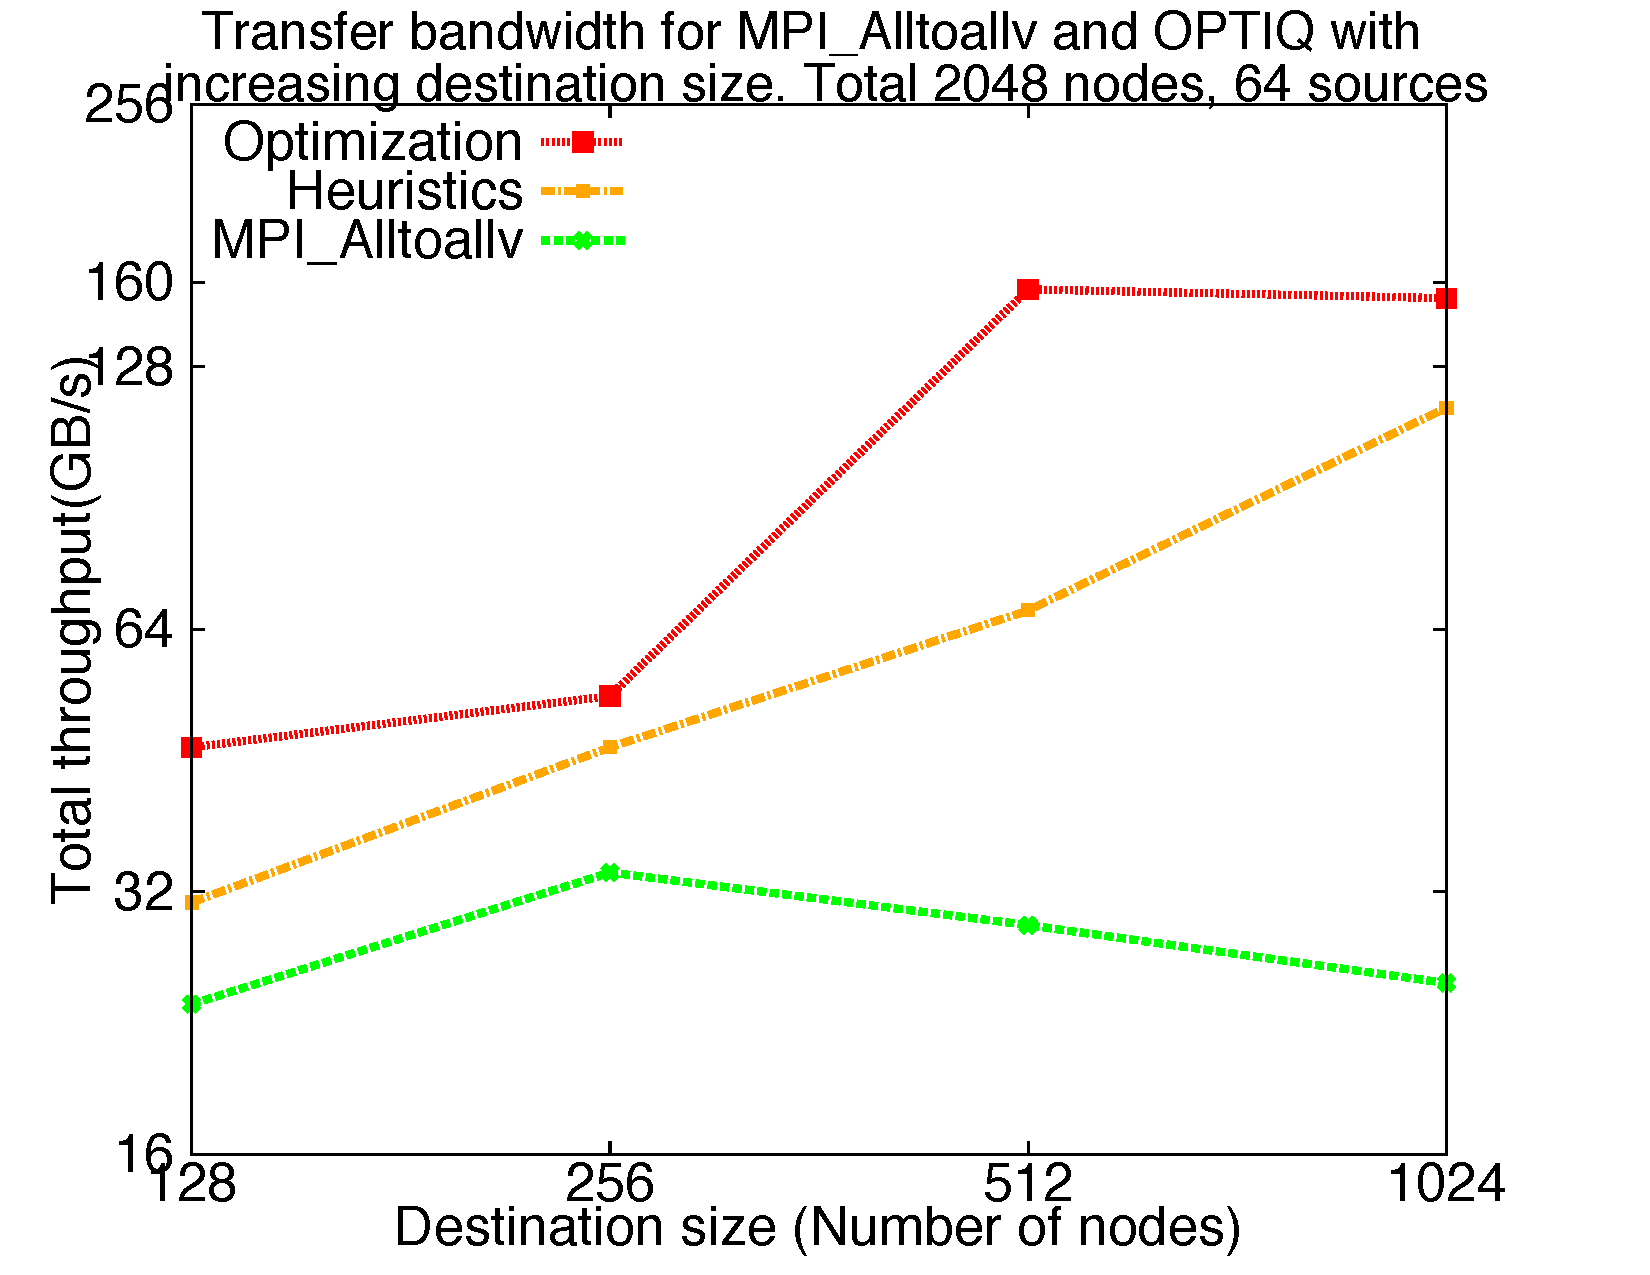
\includegraphics[width=\textwidth]{figures/incrsize_subset}
                \caption{Subset}
                \label{fig:incrsize_subset}
        \end{subfigure}
        \caption{Total data movement throughput when increasing destination size}
        \label{fig:incrsize}
\end{figure*}

\begin{table*}[!htbp]
   \centering
    \begin{tabular}{| l | p{0.5cm} | p{0.5cm} | p{0.5cm} | p{0.5cm} | p{0.5cm} | p{0.5cm} |p{0.5cm} | p{0.5cm} | p{0.5cm} | p{0.5cm} |p{0.5cm} | p{0.5cm} |p{0.5cm} | p{0.5cm} |p{0.5cm} | p{0.5cm} |}
    \hline
     Num. Dest & \multicolumn{4}{ c | }{128} & \multicolumn{4}{ c| }{256} & \multicolumn{4}{ c| }{512} & \multicolumn{4}{ c| }{1024} \\ \hline
     Patterns & {Max} & Avg & Opt Paths & Heu Paths & Max & Avg & Opt Paths & Heu Paths & Max & Avg & Opt Paths & Heu Paths & Max & Avg & Opt Paths & Heu Paths \\ \hline
     Disjoint & 15 & 9.50 & 355 & 1021 & 18 & 10.44 & 923 & 1386 & 20 & 10.44 & 1101 & 1978 & 21 & 10.19 & 1631 & 1958 \\ \hline
     Overlap  & 11 & 6.25 & 476 & 2108 & 16 & 7.19 & 937 & 2864 & 18 & 8.38 & 1690 & 4064 & 21 & 9.12 & 2081 & 4710 \\ \hline
     Subset   & 11 & 5.5  & 491 & 1799 & 16 & 6.69 & 665 & 2184 & 20 & 8.31 & 1255 & 3021 & 21 & 8.56 & 1551 & 3436\\ \hline
    \end{tabular}
    \caption{Maximum (Max) and average (Avg) distance (number of hops) and number of paths (Paths) between souces and destinations at each position.}
    \label{table:incrsize}
\end{table*}

As Figure \ref{fig:incrsize} shows, as we increase the ration between the sources and destinations by increasing the destination sizes, both of Optimization and Heuristics have better performance than MPI\_Alltoallv. In addition, they work better at scale than MPI\_Alltoallv. The throughput of Optimization approach increases for destination sizes of 256 and 512 but slightly reduces at 1024 nodes while the throughtput of Heuristic approach increases as the destination size increases.  
